%%% Realisering for optimering af reguleringsloop %%%

\subsection{Gain-fase}
Måling af systemets gain-fase karakteristik udføres på samme måde som ved 2. iteration. Opsætning af network analyzer'en er gennemgået i afsnit~\ref{gain_fase_2}. Bode plot for fejlforstærkeren er vist på figur~\ref{fig:Realisering_error_op_amp_3}, hvor der er målt over indgangen til fejlforstærkeren, og udgangen af den. Den målte forstærkning vises med blå, den målte fase er den røde, den analyserede forstærkning er den stiplede grønne, og den analyserede fase er den stiplede lilla. Det ses, at den ønskede funktionalitet af fejlforstærkeren er opnået da, henholdsvis forstærkning og fase, ligger oven i hinanden. Det betyder den ønskede forstærkning på $8.5\decibel$, ved frekvenser over $132\hertz$ er opnået. 

\begin{figure}[H]
	\center
	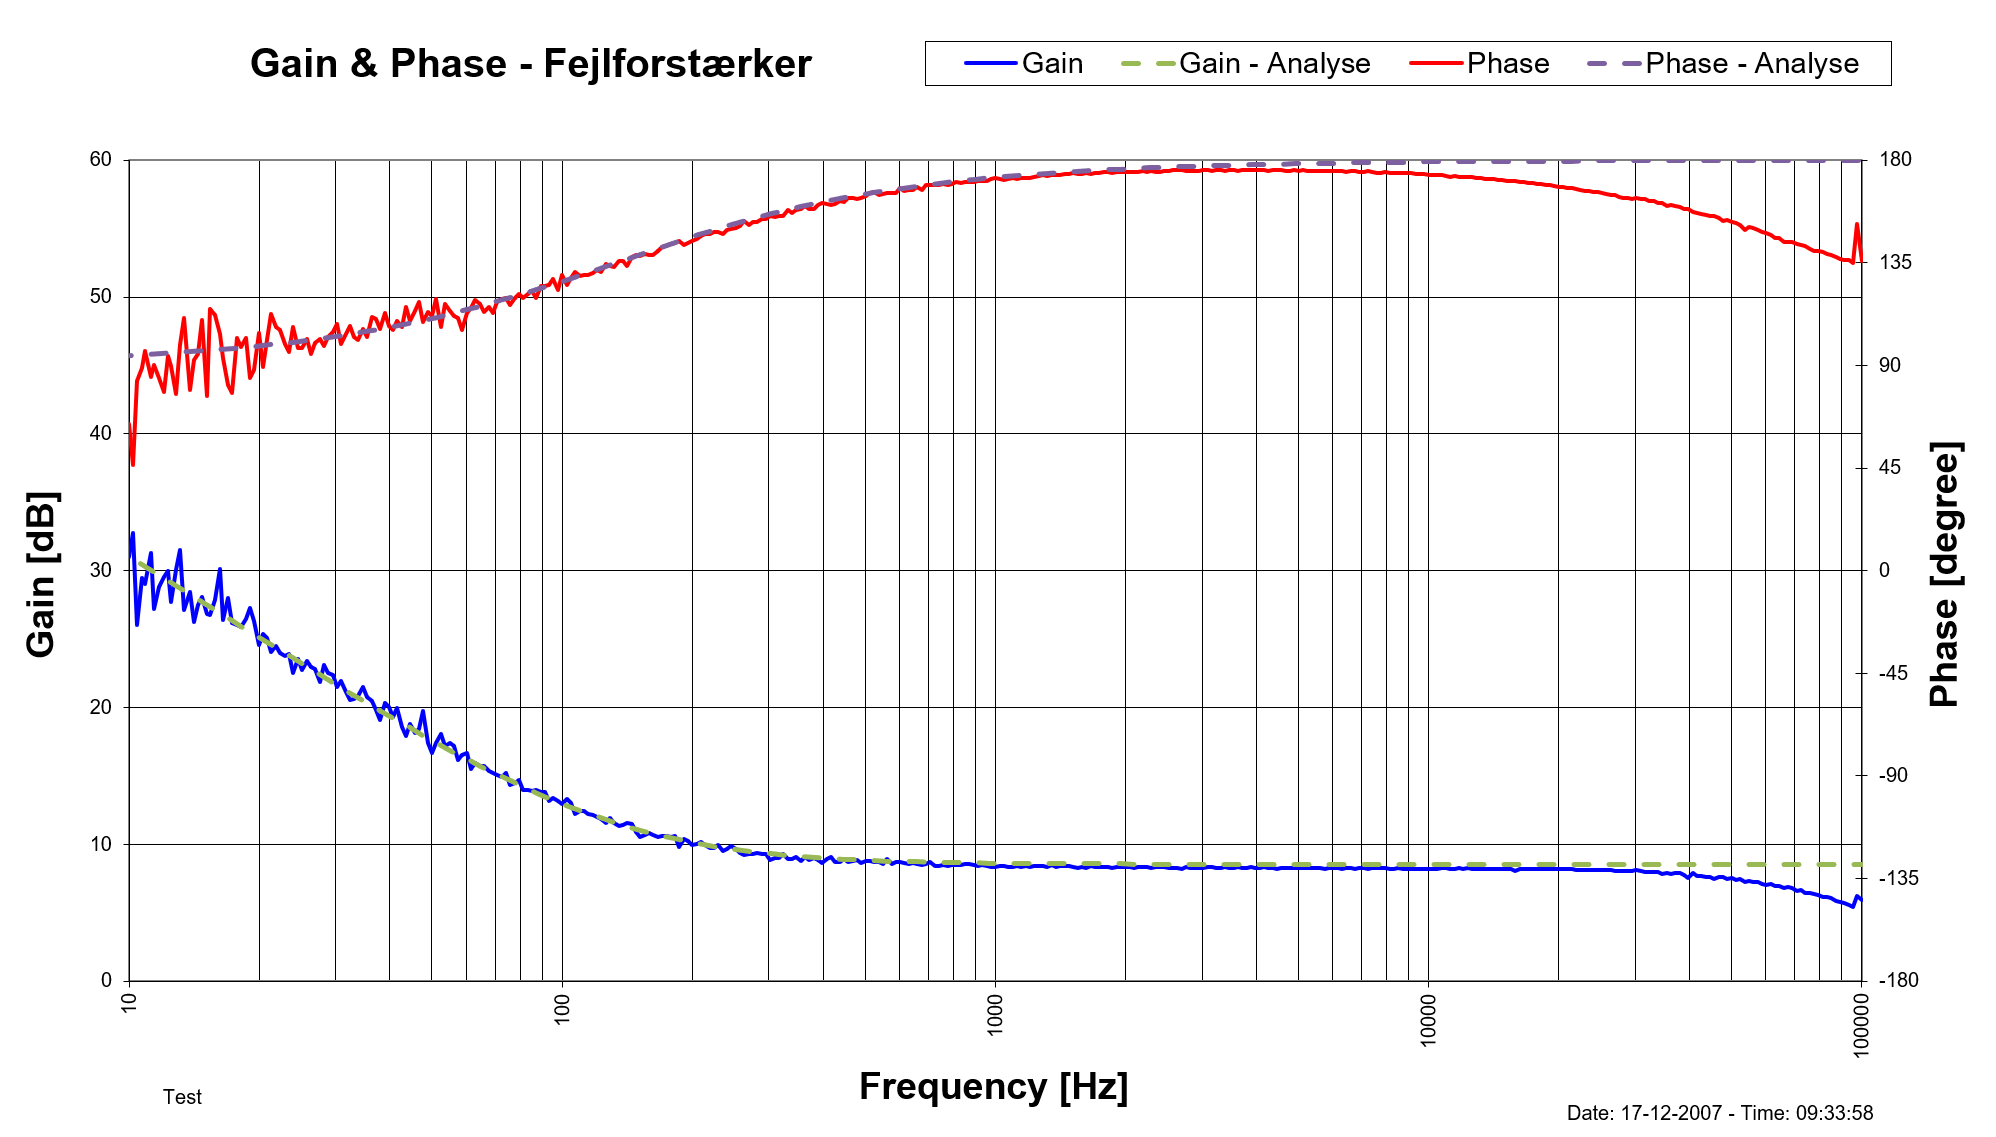
\includegraphics[max width=0.7\linewidth]{/tex/3iteration/billeder/Realisering/Realisering_gain_fase_opamp.PNG}
	\caption{Realisering af fejlforstærkeren}
	\label{fig:Realisering_error_op_amp_3}
\end{figure}

\noindent Bode plottet for det samlede system er vist på figur~\ref{fig:Realisering_total_3}. Her måles der over den modstand, hvor fejlsignalet indføres. Det svarer til at måle fra indgangen af fejlforstærkeren til udgangen af converteren. Gain for realiseringen er den blå, mens gain for analysen er den grønne stiplede. Fasen for realiseringen er den røde, mens fasen for analysen er den stiplede lilla. På bode plottet ses det, at der er en større afvigelse ved højere frekvenser. Det kan se ud til, at der er en pol i systemet, der ikke er taget højde for i analysen. Da dette sker ved frekvenser hvor gain-margin skal aflæses, bliver denne måling usikker. Den aflæses dog til $14.5\decibel$, hvilket er en afvigelse på $4.5\decibel$ ift. analysen. Fasemargin og båndbredden aflæses til henholdsvis $69.8^\circ$ og $3.86k\hertz$, hvilket stemmer med det forventede. 

\begin{figure}[H]
	\center
	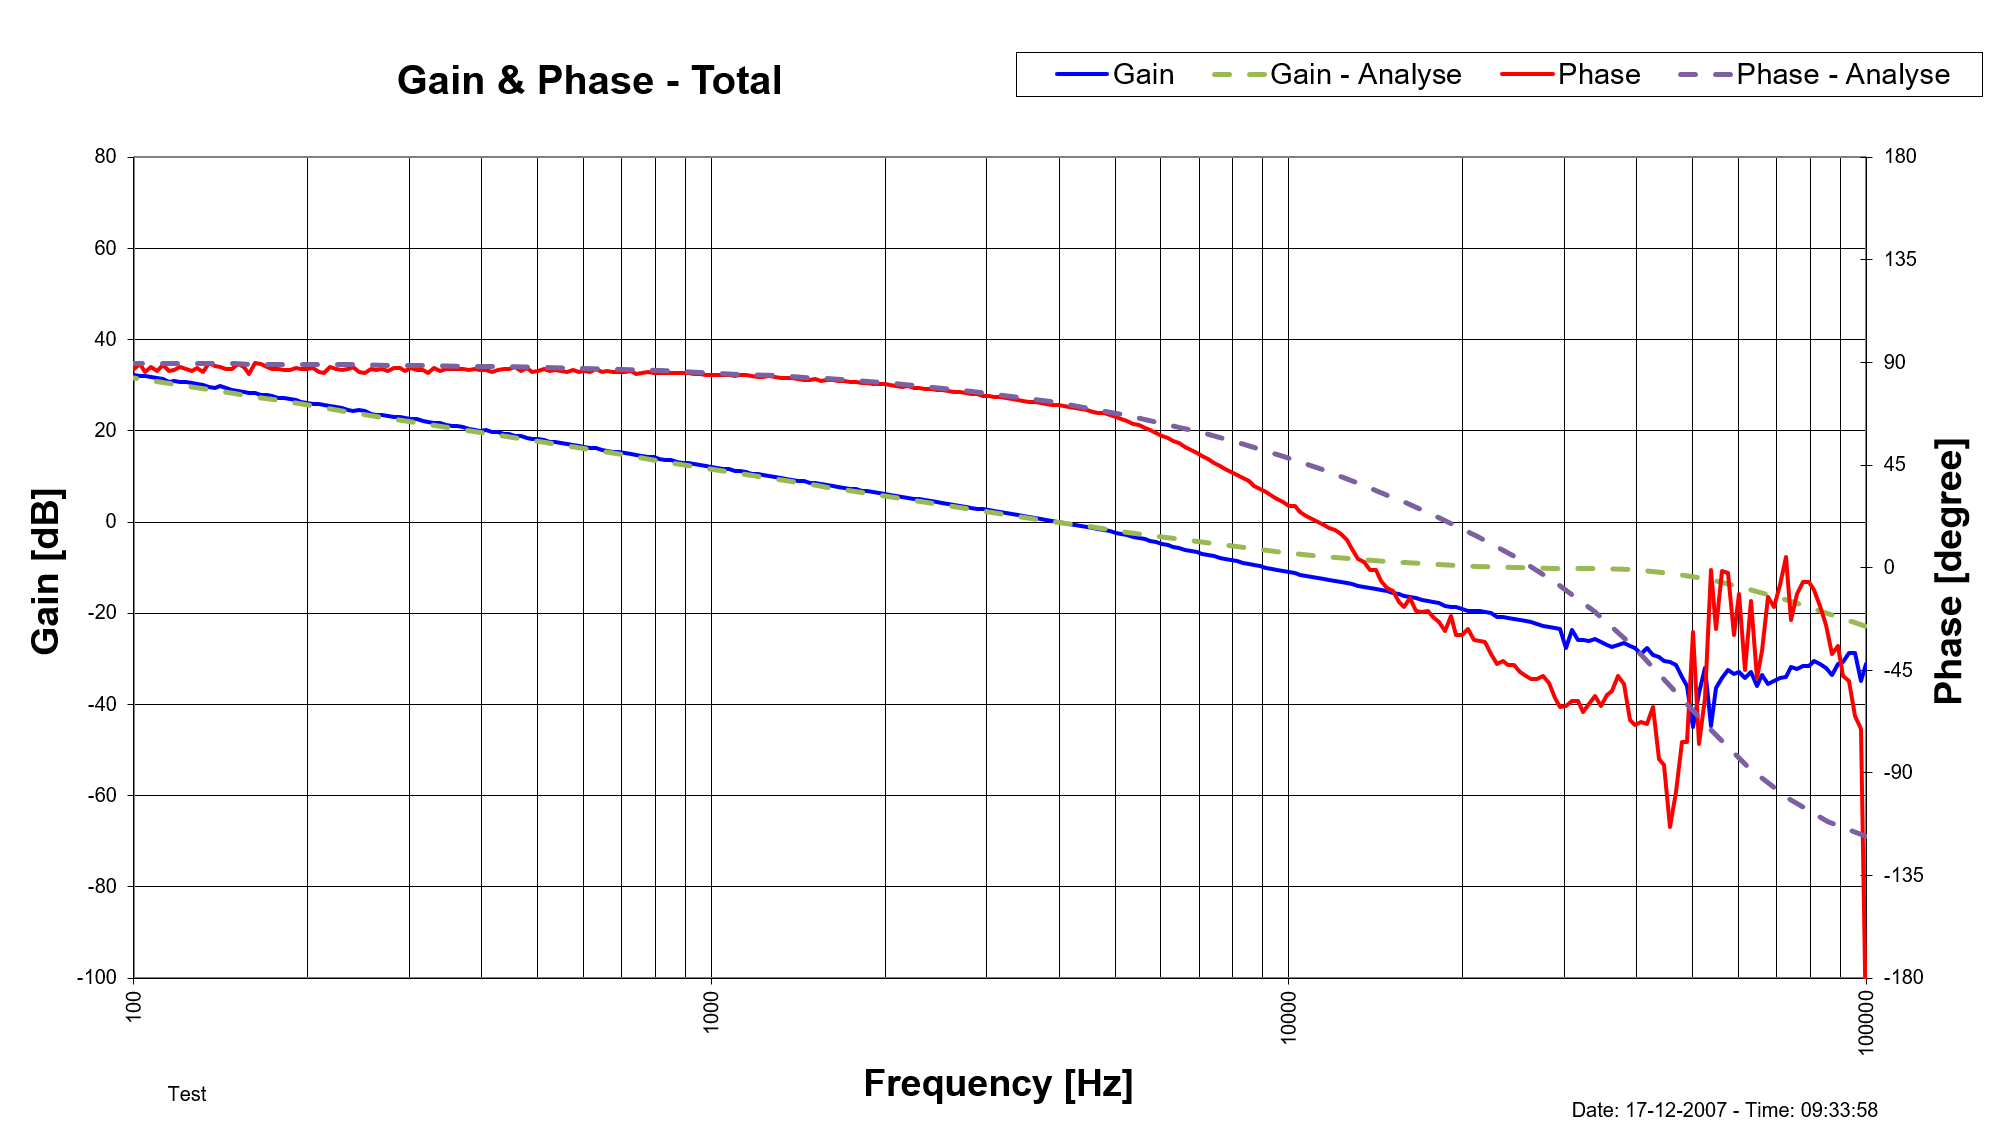
\includegraphics[max width=0.7\linewidth]{/tex/3iteration/billeder/Realisering/Realisering_gain_fase_total.PNG}
	\caption{Gain-fase måling af det samlede system}
	\label{fig:Realisering_total_3}
\end{figure}

\noindent Bode plottet for det samlede system måles også med maksimal inputspænding på 50V. Dette er vist på figur~\ref{fig:Realisering_total_50V_3}. Her er forstærkningen blå, og fasen er rød. Gain-margin aflæses til $14.3\decibel$, fasemargin aflæses til $76.3^\circ$, og båndbredden aflæses til $5.7k\hertz$. Dette viser, at systemet er stabilt ved både lav og høj inputspænding.

\begin{figure}[H]
	\center
	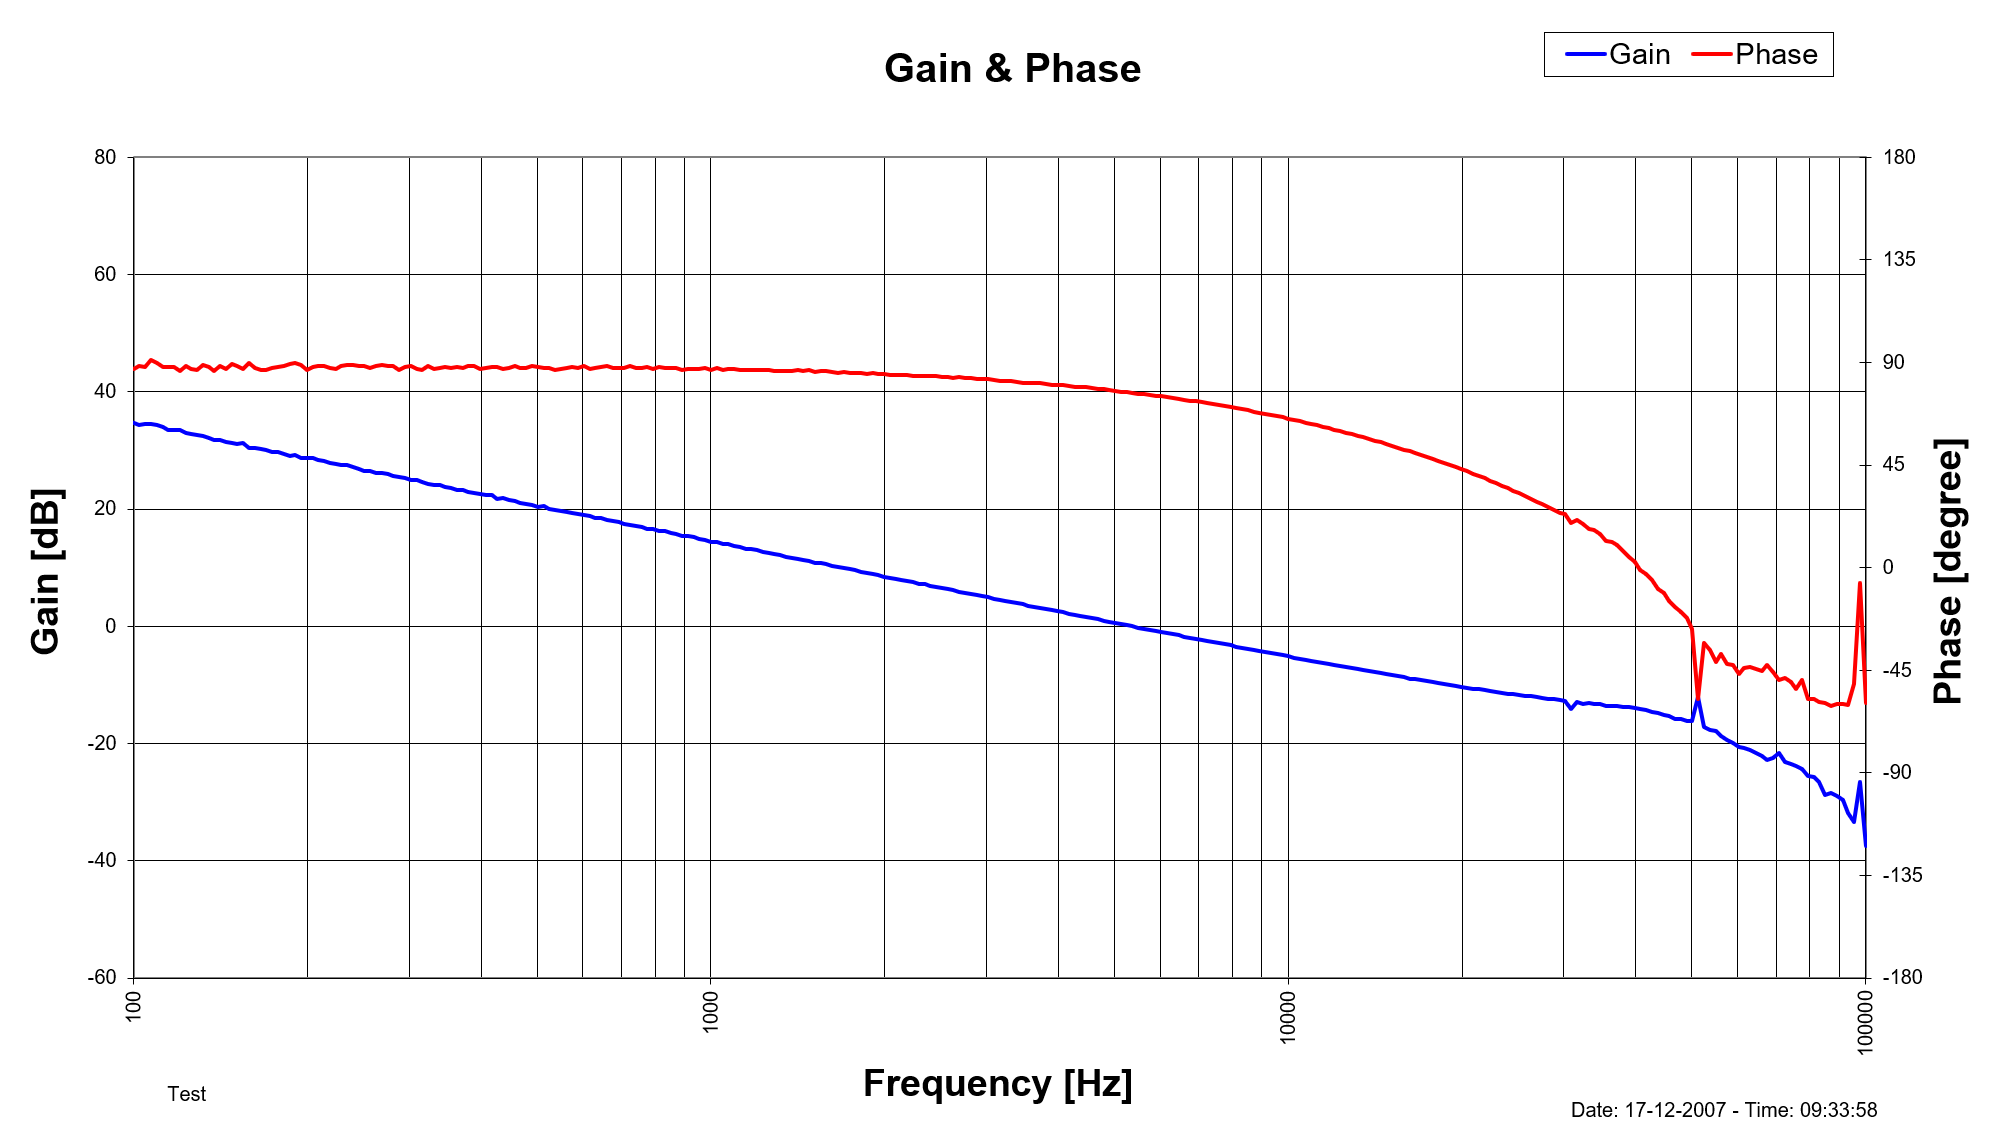
\includegraphics[max width=0.7\linewidth]{/tex/3iteration/billeder/Realisering/Realisering_gain_fase_total_50V.PNG}
	\caption{Gain-fase måling af det samlede system - 50V inputspænding}
	\label{fig:Realisering_total_50V_3}
\end{figure}





